
\medskip
Les trois questions suivantes sont indépendantes.

\begin{enumerate}
	\item $\text{A} = 2x(x - 1) - 4 (x - 1)$.
	
	Développer et réduire l'expression A.
	\item Montrer que le nombre $-5$ est une solution de l'équation \quad $(2x + 1) \times (x-2) = 63$.
	
	\item On considère la fonction $f$ définie par \quad $f(x) = -3x + 1,5$.
		\begin{enumerate}
			\item Parmi les deux graphiques ci-dessous, quel est celui qui représente la fonction $f$ ?
			
			\item Justifiez votre choix.
		\end{enumerate}
	\end{enumerate}

	\begin{tabularx}{\linewidth}{XX}
		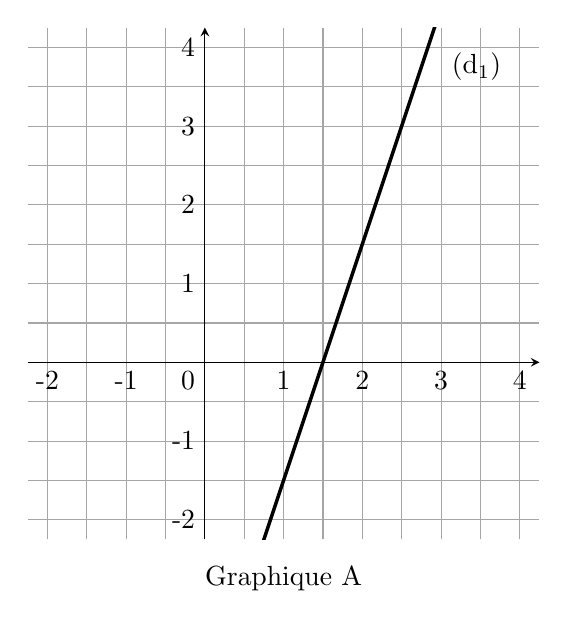
\begin{tikzpicture}[>=stealth]
		\node at(1,-2.75){Graphique A};
		 \clip (-2.25,-2.25) rectangle (4.25,4.25);
		 \draw[xstep = 0.5,ystep = 0.5, gray!70] (-2.25,-2.25) grid (4.25,4.25);
		 \draw [->] (-2.25,0) --(4.25,0);
		 \draw [->] (0,-2.25) --(0,4.25);
		 \foreach \n in {-2,-1,1,2,3,4}{
			\node at (\n,0) [below ]{\np{\n}}; 
			\node at (0,\n) [left]{\np{\n}};
	 	}
 		\node at (0,0) [below left] {0};
 		\draw[domain = 0.5:3.5,line width=1.25pt] plot (\x,{3*\x-4.5});
 		\node at (3.45,3.75) {(d$ _1 $)};
		\end{tikzpicture}&
				\hfill 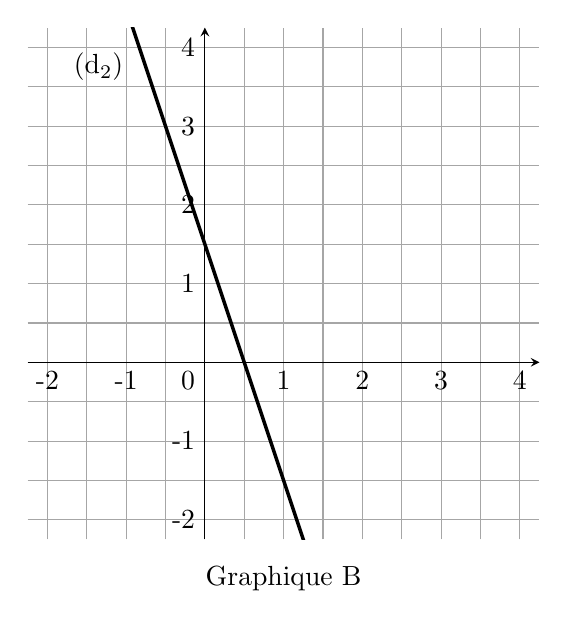
\begin{tikzpicture}[>=stealth]
		\node at(1,-2.75){Graphique B};
		\clip (-2.25,-2.25) rectangle (4.25,4.25);
		\draw[xstep = 0.5,ystep = 0.5, gray!70] (-2.25,-2.25) grid (4.25,4.25);
		\draw [->] (-2.25,0) --(4.25,0);
		\draw [->] (0,-2.25) --(0,4.25);
		\foreach \n in {-2,-1,1,2,3,4}{
			\node at (\n,0) [below ]{\np{\n}}; 
			\node at (0,\n) [left]{\np{\n}};
		}
		\node at (0,0) [below left] {0};
		\draw[domain = -1.5:1.5,line width=1.25pt] plot (\x,{-3*\x+1.5});
		\node at (-1.35,3.75) {(d$ _2 $)};
		\end{tikzpicture}
	\end{tabularx}

\vspace{5mm}

